%%%%%%%%%%%%%%%%%%%%%%%%%%%%%%%%%%%%%%%%%
% Beamer Presentation
% LaTeX Template
% Version 1.0 (10/11/12)
%
% This template has been downloaded from:
% http://www.LaTeXTemplates.com
%
% License:
% CC BY-NC-SA 3.0 (http://creativecommons.org/licenses/by-nc-sa/3.0/)
%
%%%%%%%%%%%%%%%%%%%%%%%%%%%%%%%%%%%%%%%%%

%----------------------------------------------------------------------------------------
%	PACKAGES AND THEMES
%----------------------------------------------------------------------------------------

\documentclass{beamer}

\mode<presentation> {

% The Beamer class comes with a number of default slide themes
% which change the colors and layouts of slides. Below this is a list
% of all the themes, uncomment each in turn to see what they look like.

%\usetheme{default}
%\usetheme{AnnArbor}
%\usetheme{Antibes}
%\usetheme{Bergen}
%\usetheme{Berkeley}
%\usetheme{Berlin}
%\usetheme{Boadilla}
%\usetheme{CambridgeUS}
%\usetheme{Copenhagen}
%\usetheme{Darmstadt}
%\usetheme{Dresden}
%\usetheme{Frankfurt}
%\usetheme{Goettingen}
%\usetheme{Hannover}
%\usetheme{Ilmenau}
%\usetheme{JuanLesPins}
%\usetheme{Luebeck}
%\usetheme{Madrid}
%\usetheme{Malmoe}
%\usetheme{Marburg}
%\usetheme{Montpellier}
%\usetheme{PaloAlto}
%\usetheme{Pittsburgh}
%\usetheme{Rochester}
%\usetheme{Singapore}
%\usetheme{Szeged}
\usetheme{Warsaw}

% As well as themes, the Beamer class has a number of color themes
% for any slide theme. Uncomment each of these in turn to see how it
% changes the colors of your current slide theme.

%\usecolortheme{albatross}
%\usecolortheme{beaver}
%\usecolortheme{beetle}
\usecolortheme{crane}
%\usecolortheme{dolphin}
%\usecolortheme{dove}
%\usecolortheme{fly}
%\usecolortheme{lily}
%\usecolortheme{orchid}
%\usecolortheme{rose}
%\usecolortheme{seagull}
%\usecolortheme{seahorse}
%\usecolortheme{whale}
%\usecolortheme{wolverine}

%\setbeamertemplate{footline} % To remove the footer line in all slides uncomment this line
%\setbeamertemplate{footline}[page number] % To replace the footer line in all slides with a simple slide count uncomment this line

\setbeamertemplate{navigation symbols}{} % To remove the navigation symbols from the bottom of all slides uncomment this line
}

\usepackage{graphicx} % Allows including images
\usepackage{booktabs} % Allows the use of \toprule, \midrule and \bottomrule in tables
\usepackage{hyperref}
\hypersetup{
	colorlinks=true,
	linkcolor=blue,
	filecolor=magenta,      
	urlcolor=cyan,
	citecolor=black,
}

%----------------------------------------------------------------------------------------
%	TITLE PAGE
%----------------------------------------------------------------------------------------

\title{Lucene Spatial Index} % The short title appears at the bottom of every slide, the full title is only on the title page

\author{
Alix Bernard
} % Your name
\institute % Your institution as it will appear on the bottom of every slide, may be shorthand to save space

\date{\today} % Date, can be changed to a custom date

\begin{document}

\begin{frame}
\titlepage % Print the title page as the first slide
\end{frame}

\begin{frame}
\frametitle{Overview} % Table of contents slide, comment this block out to remove it
\tableofcontents % Throughout your presentation, if you choose to use \section{} and \subsection{} commands, these will automatically be printed on this slide as an overview of your presentation
\end{frame}

%----------------------------------------------------------------------------------------
%	PRESENTATION SLIDES
%----------------------------------------------------------------------------------------

%------------------------------------------------
\section{Main indexing methods} % Sections can be created in order to organize your presentation into discrete blocks, all sections and subsections are automatically printed in the table of contents as an overview of the talk
%------------------------------------------------

% \subsection{Subsection Example} % A subsection can be created just before a set of slides with a common theme to further break down your presentation into chunks

\begin{frame}
\frametitle{Main indexing methods}
In DBMS, data is stored as records where very records has a key field that helps recognizing it uniquely. Indexing is a data structure technique which aims to efficiently retrieve those records based on some attributes on which the indexing is done. Multiple types of indexing exists, the main ones are display in figure 1.

\begin{figure}[h]
	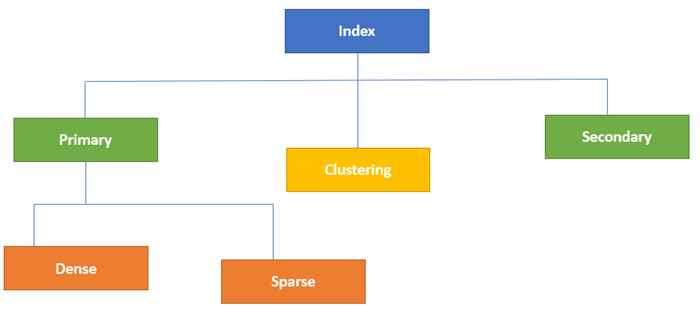
\includegraphics[scale=.25]{main_indexes.png}
	\caption{1 Main indexes}
\end{figure}
\end{frame}


%------------------------------------------------
\section{Spatial indexing}
%------------------------------------------------

\begin{frame}
\frametitle{Spatial indexing}
When dealing with spatial data, it is apparent that traditional indexing is not fitted for the task, therefore spatial indexing has been created.

Spatial data (aka geospatial data or geographic information) is data identifying geographic location of features and boundaries --- usually on earth. It is usually stored as coordinates and topology, and is data that can be mapped.
\end{frame}

\begin{frame}
\frametitle{Spatial indexing}
Spatial data is composed of three general data types: point, line, and region; furthermore they are differentiated in two classes: simple and complex.

\begin{figure}[h]
	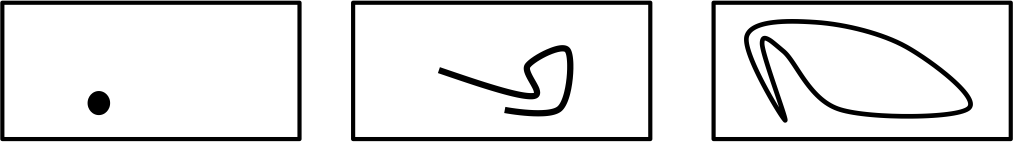
\includegraphics[scale=.3]{simple_spatial_types.png}
	\caption{2.1 Simple spatial type}
\end{figure}

\begin{figure}[h]
	
\includegraphics[scale=.3]{complex_spatial_types.png}
	\caption{2.2 Complex spatial type}
\end{figure}
\end{frame}

\begin{frame}
\frametitle{Spatial indexing}
One way to index those data is to index their bounding boxes; therefore when performing a search such as "which lines cross this area?", only the question "which bounding boxes overlap this bounding box?" is answer at first using the indexing since it is a really fast operation, afterwards an exact calculation is performed to answer the initial question accurately.

\begin{figure}[h]
	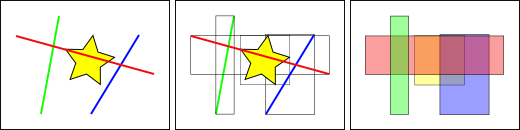
\includegraphics[scale=.5]{example_bounding_boxes.png}
	\caption{3 Example of bounding boxes}
\end{figure}
\end{frame}



%------------------------------------------------
\section{Lucene Spatial indexing}
%------------------------------------------------

\begin{frame}
\frametitle{Lucene Spatial indexing}
One way to index spatial data is to use the Lucene Spatial indexing that uses the Lucene engine to perform a spatial search.

The Lucene engine (Apache LuceneTM), is a full-featured text search engine library written entirely in JAVA. This engine has a module allowing the implementation of a spatial strategy which encapsulates an approach to indexing and searching based on shapes. Different implementation of the spatial strategy will support different features.
\end{frame}


%------------------------------------------------
\section{Relevant links}
%------------------------------------------------

\begin{frame}
For more details and examples:
\begin{thebibliography}{00}
	\bibitem{b1} https://lucene.apache.org/core/4\_0\_0/spatial/
	\bibitem{b2} https://orientdb.com/docs/3.0.x/indexing/Spatial-Index.html
	\bibitem{b3} https://postgis.net/workshops/postgis-intro/indexing.html\#how-spatial-indexes-work
\end{thebibliography}
\end{frame}
%----------------------------------------------------------------------------------------

\end{document} 
